\begin{document}
\section{Methodology}
\subsection{Project Aim}
The principle aim of this project was to create a Distributed Platform Architecture that can be utilised for Machine Learning Applications. The project was targeted to be developed on an existing platform at Embedded System Lab in University of Auckland. Implementation was split between the two members of this group and a breakdown of the common aims and specific aims can be found in the Appendix.


\subsection{Platform Development}

\subsubsection{Multitier Architecture}     
    \begin{flushleft}
        As shown in Figure \ref{fig:Multi-tier Platform}, a multi-tier platform was developed for big-data analytics. This platform is continuously being developed by research projects in the Embedded Systems Lab at The University of Auckland. The pre-existing platform aimed to segregate operations through a multi-tier architecture of gateway and fog level computing. The fog layer has three clusters, of which two are classified as streaming clusters and one as an analytics cluster.  
        
        \begin{figure}[H]
      
          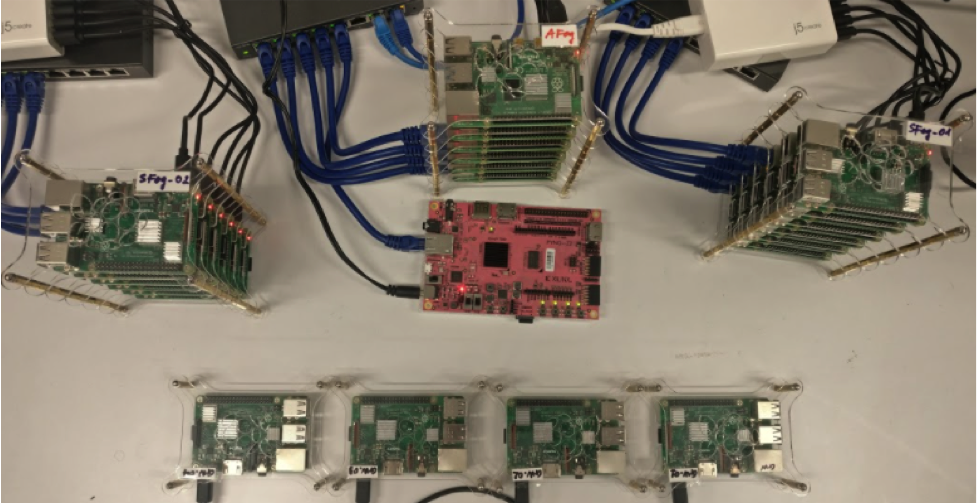
\includegraphics[width=\textwidth]{images/MultitierPlatform.png}
          \caption{Multi-tier Platform}
          \label{fig:Multi-tier Platform}
        \end{figure}
        
    \end{flushleft}

    
\subsubsection{Gateway Layer}     
    \begin{flushleft}
        The gateway layer  is used to replicate the behaviour of  car park zones (with multiple sensors in a zone). It uses a Java simulator program created in a past research project which estimates the parking occupancy of a zone within a carpark. As shown in Figure \ref{fig:Gateway Layer}. There are 4 nodes in the gateway layer. Each node is a Raspberry Pi 3B+.
           
        \begin{figure}[H]
          
          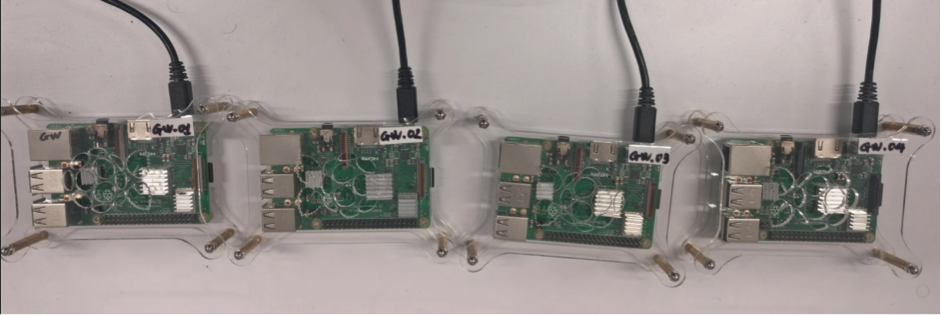
\includegraphics[width=\textwidth]{images/GatewayLayer.png}
          \caption{Gateway Layer}
          \label{fig:Gateway Layer}
        \end{figure}
        
    \end{flushleft}

\subsubsection{Fog Layer} 
       
    
    \begin{flushleft}
        
        The fog layer consists of 2 types of clusters, S-Fog for streaming and A-Fog for big data analytics. There are 2 S-Fog clusters made up of six Raspberry Pi’s which are used to collect car park data from the gateway nodes, pre-process it and store the records on HDFS. There is an A-Fog cluster which is developed for the purposes of this project. It consists of four Raspberry Pi 4B devices (4GB RAM) as shown in Figure ~\ref{fig:RPi Cluster} . There are two nodes used for Apache Kafka which are not utilized by this project. As the development process was conducted, the A-Fog cluster was revised to increase development agility, speed of inference and provide a stable platform. This is detailed in the following section.
        \begin{figure}[H]
      
          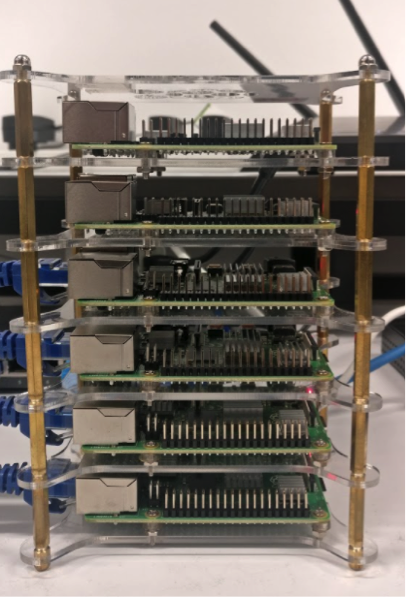
\includegraphics[scale=0.8]{images/RpiCluster.png}
          \caption{RPi Cluster}
          \label{fig:RPi Cluster}
        \end{figure}
     
    \end{flushleft}
    
\subsubsection{A-Fog Layer}
    \begin{flushleft}
        \begin{figure}[H]
          
              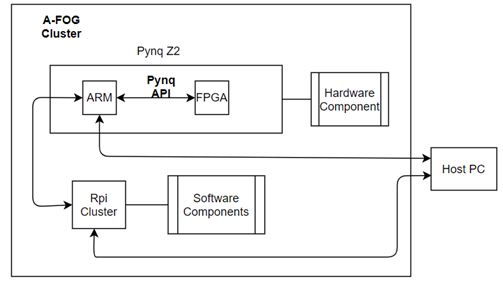
\includegraphics[scale=0.8]{images/A-Fog.JPG}
              \caption{A-Fog}
              \label{fig:A-Fog}
        \end{figure}
        
        As shown in Figure \ref{fig:A-Fog}, the A-Fog Layer is partitioned into Hardware and Software Components. The system consists of a raspberry pi cluster (Rpi Cluster), a Host PC and a Pynq Board which serves as the Hardware Inference Engine. These are connected via a network switch using RJ45 ethernet cables. Apache Spark is the unifying platform which is run by all the components in the A-Fog as part of a Distributed System. The ARM processor on the Pynq runs Linux along with Apache Spark. Jupyter Notebooks is a tool used commonly for datascience in industry The FPGA fabric is controlled using python APIs and applications in python developed on a Jupyter Notebooks environment which can accessed on the Host PC. The RPi cluster uses the Raspbian OS and runs Apache Spark along with Apache HDFS. It consists of a Master Node and three Worker Nodes. The Master Node deploy machine learning applications to the worker nodes, doing so in a distributed way. 

        
        Host PC -  Runs Linux with Apache Spark and contains all the tools used to develop the software programs to train a Machine Learning Model (Neural Network) and deploy them to the RPi Cluster. These include the following tools.
         
        
    \end{flushleft}
    

\begin{itemize}
    \item Apache Hadoop Distributed File Storage (HDFS), a distributed file storage system used to store datasets for training, pre-trained models and untrained models.  
    
    \item HLS4ML, an open source tool used to convert pre-trained Keras models to a high level synthesis (HLS) vivado project. 
    
    \item The Vivado Design Suite, to convert the HLS project into a bitstream which can be programmed onto the FPGA on the Pynq board.  
    
    \item IDE’s such as IntelliJ and PyCharm to aid in software development.  
    
   
\end{itemize}

\subsubsection{Big Picture}

Outlined is a general overview of how this platform is intended to be used.  
    \begin{figure}[H]
          
      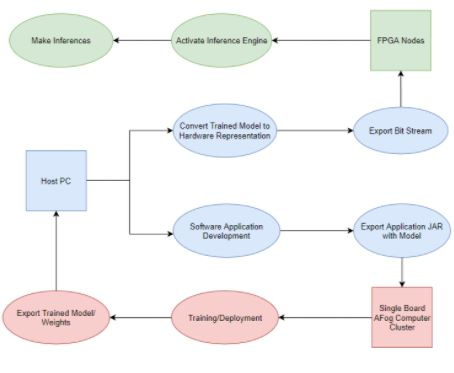
\includegraphics[scale=0.8]{images/BigPicture1.JPG}
      \caption{Big Picture}
              
    \end{figure}

%
%
%
\subsection{ Selection of Machine Learning Frameworks}
    \begin{flushleft}
    There are several frameworks which can be used to train machine learning models on a distributed cluster using Apache Spark. The frameworks considered in this project were Spark MLlib, Intel Analytics Zoo and Deep Learning For Java (DL4J). All these frameworks were investigated for the purpose of developing a machine learning algorithm to solve the problem of predicting car park occupancy in the short and long term. 
    \end{flushleft}
 
    \subsubsection{Spark MLlib}
        \begin{flushleft}
        This framework is provided by default as part of the Data Analytics layer of Apache Spark. Hence it inherits all the features of Apache Spark such as being polyglot. It is written in Scala and is one the few libraries that is able to utilise accelerator awareness with Spark 3.0+. Accelerator Awareness is aimed at distributed systems where some operations can be offloaded to GPU or FPGA to increase performance. The disadvantages of this library is lack of suitable algorithms for machine learning. The number of available models are limited, especially in the area of neural networks. This library has a multilayer perceptron model available only for classification problems, which will not solve the problem of predicting parking occupancy as it is a regression problem. Visualisation tools are also quite limited, although external Python libraries such as Matplotlib can be used.However, using external python libraries or user defined functions will affect performance so there is a tradeoff between visualisation and speed. An important feature provided in this framework are Spark ML pipelines, which allow the machine learning process to be automated.  
        \end{flushleft}
 
    \subsubsection{Analytics Zoo}
        \begin{flushleft}
        This framework is an open source tool originally developed by Intel. It is also polyglot, with API documentation provided for Scala and Python. The tool aims to scale popular frameworks for machine learning to distributed big data problems. The frameworks supported are Tensorflow,Caffe,Pytorch and Keras. Keras is a high level API which allows programmers to develop neural networks which can run on any of the aforementioned frameworks.Analytics Zoo has APIs for Keras which can be used in combination with Spark ML pipelines to automate the machine learning process. Analytics Zoo features a range of models and algorithms which allows developers to quickly prototype machine learning solutions. It also supports visualisation of the machine learning process via Tensorboard, which is crucial to ease of development. An important use case in the machine learning space is cross validation which can be made part of the Spark ML pipeline. Analytics Zoo utilizes the SparkSQL data type for all operations, which significantly improves the performance. An overview of Analytics Zoo functionality is shown below. The main disadvantage of Analytics Zoo is that it uses Intel Math Kernel Library (MKL) for operations. This library is not compatible with processors with ARM architecture, it only supports select Intel processors (most common is Intel x86\_64 architecture) supported. This means that any distributed training or inference program cannot be deployed to the Raspberry Pi cluster, as they use ARM processors. This is a major drawback of Analytics Zoo, considering that most  low cost embedded devices use ARM processors.  
         \end{flushleft}
        
       
     
        \begin{figure}[H]
              
          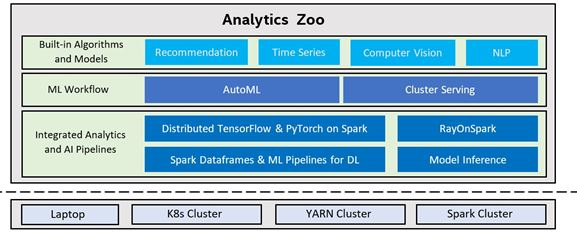
\includegraphics[scale=0.8]{images/AnalyticsZoo.JPG}
          \caption{Analytics Zoo Architecture}
          \label{fig:AnalyticsZoo}
                  
        \end{figure}
    \subsubsection{DL4J}
        \begin{flushleft}
          DL4J is an open source tool developed by Eclipse. It is also polyglot, with APIs in Java and Scala. It is designed to run independently of Apache Spark. An important distinction between DL4J and the other frameworks explored is that DL4J does not integrate well with Spark tools such as ML pipelines. It also does not support the Spark SQL datatype and instead relies on external libraries such as ND4J and Datavec,which makes development more difficult. The framework itself is not very stable, with major issues listed on its main repository. A major reason is issues with stable releases due to problems with dependency management. An advantage of DL4J is that it can be configured to use different libraries for mathematical operations such as Intel MKL and OpenBLAS. This allows DL4J programs to be deployed onto the Raspberry Pi cluster by using OpenBLAS, which is compatible with ARM architectures unlike Intel MKL. There is a certain level of integration when importing models with existing frameworks such as Tensorflow, but this is limited and not as extensive compared to Analytics Zoo.
        \end{flushleft}  
    \subsubsection{Comparison of Frameworks}    
        
        \begin{flushleft}
            The frameworks are ranked according to criteria as shown below. The principle that is taken into consideration while choosing the appropriate framework is to prioritise lower development time compared to lower training time. Hence, Analytics Zoo is found to be the best fit solution to solve not only the parking occupancy problem, but many other machine learning problems such as image classification. 
        \end{flushleft}
        
        \begin{figure}[H]
              
              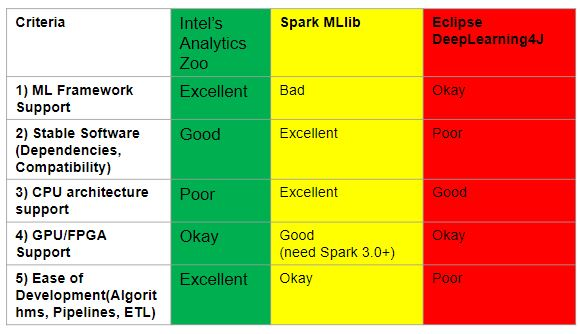
\includegraphics[scale=0.8]{images/ComparisonTable.JPG}
              \caption{Big Picture}
              \label{fig:Big Picture}
                  
            \end{figure}

\subsection{Implementation of Machine Learning Model}
    The machine learning model, defined as a Feed-Forward Neural Network (NN), is trained in a recurring loop, which has a certain number of iterations (commonly referred to as Epochs). There are three parts of an NN which are the input layer, hidden layer/s and the output layer, as shown in a general diagram below. Training Data is fed through the input layer. Each input parameter is a Node/Neuron. There are three densely connected hidden layers (Dense Layer - Each neuron in a layer is connected to all the neurons in adjacent layers by a weight). Each hidden layer contains five neurons. The output value of each Neuron N is described by the equation below. The output layer will give the predicted value. The black box view of the parking prediction model (Neural Network) is shown. The activation function currently used is Relu. In future, different Activation functions can be used to model non-linear behavior.
    
        \begin{figure}[H]
              
              \includegraphics[scale=0.8]{images/MLModel.JPG}
              \caption{MLModel}
              \label{fig:MLModel}
                  
        \end{figure}


\subsection{Training Machine Learning Model using Apache Spark}
%% TODO ADD PIC AND REWRITE
The following steps are undertaken to train the model. The software programs to conduct the steps are implemented using the Host PC.

\begin{itemize}
    \item Convert Data Format: A Java simulator in generates ‘random’ parking occupancy data every minute (between 40\%-
    60\% occupancy level). Data generated from the simulator is stored on the HDFS in JSON format, with a file for each
    data record. For ease of processing, this is converted to a .CSV format, making it easier to extract data from. The .CSV format will also be stored onto the HDFS.  
    
    \item Define the model: Define the Neural Network using the Sequential API of TensorFlow. After adding all the layers with
    their respective activation function, the model is compiled with an optimization function. The compiled model
    architecture is saved in a.h5 format on HDFS. 
    
    \item Import Training Data: Import the data and convert the Spark timestamp to a format that the machine learning model
    can understand. After converting the Spark timestamp to Unix timestamp (32-bit unsigned integer), ‘assemble’ the
    features. This means grouping all features (Unix Timestamp and Car Park ID) together as the parameters and assigning
    the parking occupancy as the label. 
    
    \item Load into Software Framework: The .h5 model (untrained) is imported by the software frameworks (Analytics Zoo/DL4J) and converted to their own model. The software program can set hyperparameters such as Max Epochs, Optimisation Function, Batch Size etc. The model is then trained on the Training Data using distributed training APIs. Upon training, the model weights are exported and stored on HDFS.The weights can be extracted and imported by a TensorFlow model if the user wishes to deploy to the hardware accelerator for inferencing. Alternatively, the trained model can be used to inference using the RPI Cluster.
    
   
\end{itemize}










\end{document}